\subsection{Validation and Testing Procedures for Model Evaluation}\label{subsec:validation_testing_procedures}
This section describes the validation and testing procedures our experiments follow.
Selecting appropriate testing procedures is crucial for ensuring the validity and reliability of the results.
For that reason, we delineate a methodological approach that ensures our models are accurate and generalizable.

We have chosen to test and evaluate all our experiments using both cross-validation and a separate test set.
Evaluating results solely on the test set could lead to models that are overly specialized to the test set.
This occurs when searching for the optimal configuration of hyperparameters specifically tailored to the test set.
However, our objective is to develop models that demonstrate high accuracy and robustness, even on entirely unseen data.
To achieve this, we employ k-fold cross-validation to ensure our models have high generalizability, thereby increasing the likelihood that they will perform as expected on new data.

We use an $80\%/20\%$ split for training and testing sets. The training set is further subdivided into $k$ folds, which are used for cross validation.

While we employ conventional techniques like holdout sets and k-fold cross validation, \gls{libs} data imposes additional challenges to the process.

One of the primary challenges is preventing data leakage.
As per concentration matrix $\mathbf{C}$ in Section~\ref{sec:problem_definition}, each target only has one ground truth concentration value per oxide.
However, each target is shot at multiple locations, resulting in multiple instances of the same target in the dataset, as shown in Table~\ref{tab:final_dataset_example}.
Although the intensity values vary for each location, they fundamentally represent different measurements of the same target.
If we were to randomly split the dataset, some locations from a target could end up in the testing set while others remain in the training set.
This would cause data leakage, as the testing set would no longer consist solely of unseen targets.
To prevent this, we ensure that each target is represented only once in the dataset by grouping data from all locations on a given target.

Furthermore, the limited availability mentioned in Section~\ref{sec:problem_definition} of data poses another significant challenge due to the difficult collection process.
The dataset we use consists of 408 samples. This is a large dataset by \gls{libs} standards.
However, despite this, there are only a few samples with extreme concentration values for the oxides in the targets.
These extreme values present concentrations significantly different from the rest of the data points. 

When performing a random split of the dataset into multiple folds for cross-validation, as well as for training and testing sets, this small number of extreme values can result in an uneven distribution.
The presence or absence of these extreme values in any given fold can heavily influence the model's performance metrics.
If extreme values are disproportionately allocated to either the training or testing sets, the resulting model may struggle to generalize accurately.
This uneven distribution can lead to models that perform well on the majority of the data but fail to predict accurately for these extreme concentration values, which are critical in many practical applications.

\begin{figure*}[h!]
    \centering
    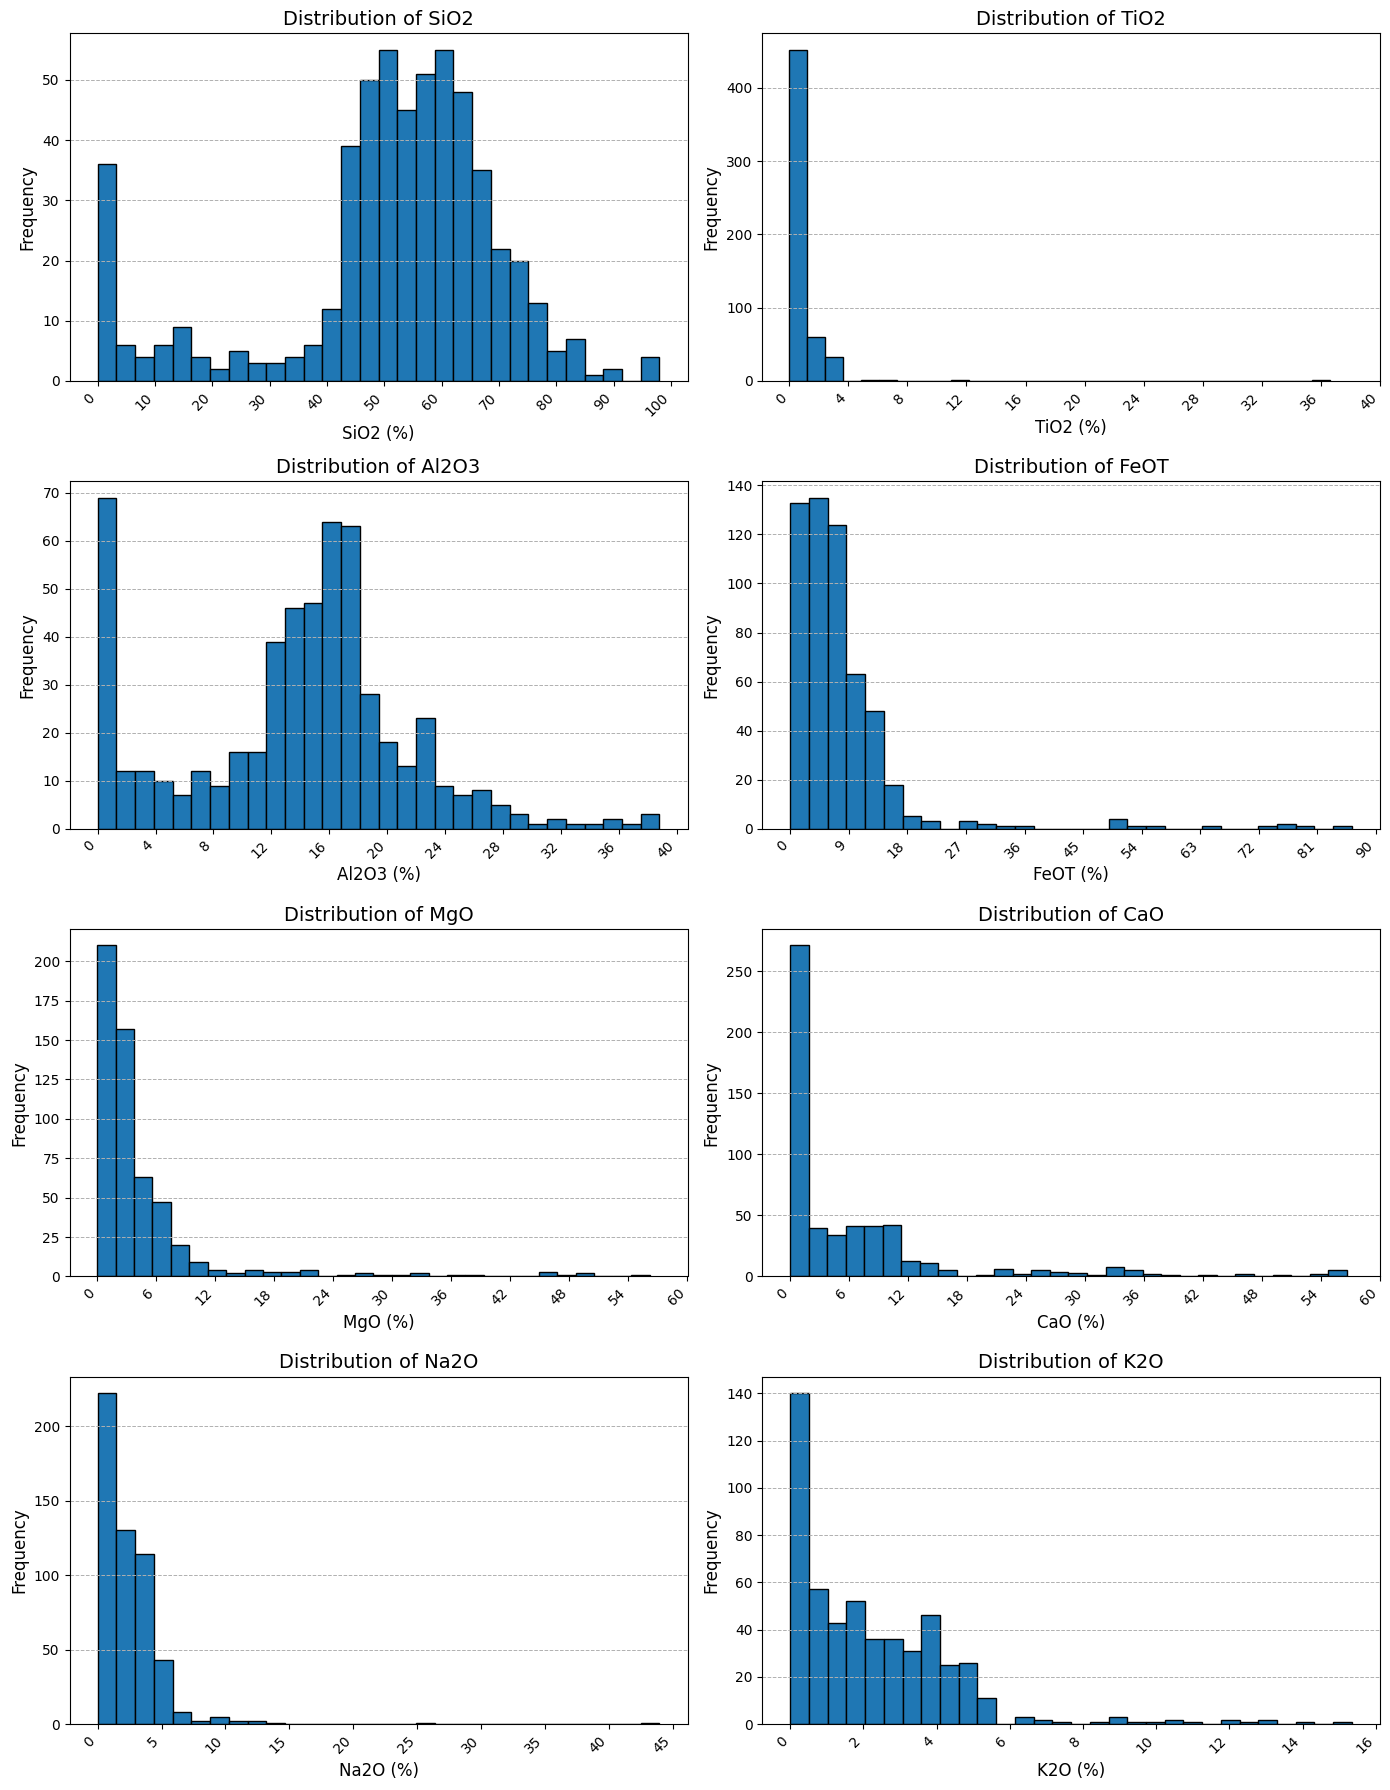
\includegraphics[width=\textwidth]{images/oxide_distributions.png}
    \caption{Distributions of various oxide concentrations in the dataset. The histograms show the frequency of concentration values for \ce{SiO2}, \ce{TiO2}, \ce{Al2O3}, \ce{FeO_T}, \ce{MgO}, \ce{CaO}, \ce{Na2O}, and \ce{K2O}.}
    \label{fig:oxide_distributions}
\end{figure*}

Figure~\ref{fig:oxide_distributions} illustrates the distributions of various oxide concentrations in our dataset.
Across all oxides, there is a general pattern of skewed distributions, with concentrations heavily weighted towards lower values.
This is particularly notable in \ce{TiO2}, \ce{FeO_T}, \ce{MgO}, \ce{CaO}, and \ce{Na2O}.
\ce{SiO2} and \ce{Al2O3} show more variability, with \ce{SiO2} exhibiting a bimodal distribution.
These distributions confirm the presence of extreme values across all oxides, which are significantly overrepresented or underrepresented, further complicating the model training process.

This necessitates careful dataset partitioning to ensure that the model training process accounts for these challenges, improving the generalizability and robustness of the models.


\subsubsection{Dataset Partitioning}\label{subsubsec:dataset_partitioning}
To ensure rigorous evaluation of our models and to address the challenges of data leakage and uneven distribution of extreme values, we have implemented a customized k-fold cross-validation procedure.
This procedure ensures that all data points from a given target are either entirely in the training set or the test set, overcoming the challenge of data leakage we mention above.
Additionally, it ensures that extreme values are handled appropriately to maintain an even distribution across folds, as demonstrated by the data distributions in Figure~\ref{fig:oxide_distributions}.

\begin{algorithm}
\caption{Custom k-Fold Cross-Validation with Extreme Value Handling}
\begin{algorithmic}[1]
\Require Dataset \( \mathbf{D} \), group column \( g \), target column \( t \), number of splits \( k \), percentile \( p \), random seed \( \textit{seed} \)
\Ensure Cross-validation folds \( \mathbf{F}_\text{cv} \), training set \( \mathbf{D}_\text{train} \), and test set \( \mathbf{D}_\text{test} \)
\State \label{line:seed} Set random seed for reproducibility if \(\text{seed} \) is not None
\State \label{line:remove_duplicates} Remove duplicate entries based on \( g \) and sort by \( t \)
\State \label{line:assign_folds} Assign fold numbers sequentially from 0 to \( k-1 \) to unique targets
\If{extreme values handling is enabled}
    \State \label{line:identify_extremes} Identify extreme values at percentiles \( p \) and \( 1-p \)
    \State \label{line:reassign_extremes} Reassign extreme values to folds \( 0 \) to \( k-2 \)
\EndIf
\State \label{line:merge_folds} Merge fold assignments back into the original dataset
\State \label{line:split_dataset} Split dataset into test set \( \mathbf{D}_\text{test} \) (fold \( k-1 \)) and remaining data \( \mathbf{D}_\text{train} \)
\State \label{line:create_folds} Create \( k-1 \) training and validation folds
\For{each fold \( i \) from 0 to \( k-2 \)}
    \State \( \mathbf{F}_\text{train}[i] \gets \mathbf{D}_\text{train} \setminus \text{fold}_i \)
    \State \( \mathbf{F}_\text{val}[i] \gets \text{fold}_i \)
    \State Append \((\mathbf{F}_\text{train}[i], \mathbf{F}_\text{val}[i])\) to \(\mathbf{F}_\text{cv}\)
\EndFor
\State \label{line:remove_fold_column} Remove fold column from all datasets
\State \Return \( \mathbf{F}_\text{cv}, \mathbf{D}_\text{train}, \mathbf{D}_\text{test} \)
\end{algorithmic}
\end{algorithm}

The procedure begins by setting a random seed for reproducibility if one is provided (Line~\ref{line:seed}).
This ensures that the results are consistent across different runs of the algorithm.
Next, the dataset is processed to remove any duplicate entries based on the group column and then sorted by the target column (Line~\ref{line:remove_duplicates}).
This step ensures that each group is uniquely identified and ordered appropriately.
The dataset we illustrate in Table~\ref{tab:final_dataset_example} would require a group column $g$ of "\texttt{Target}" to group the data by target.
The target column $t$ refers to the column with the target variable, which would be the oxide for which we are predicting the concentration, for example, \ce{SiO_2}.
By sorting the dataset by the target column, we ensure that the data is ordered by the target concentration values in ascending order.

Fold numbers are then assigned sequentially using a modulo operation to ensure a random-like distribution of the unique targets across the folds (Line~\ref{line:assign_folds}).
This means that while the assignment process follows a sequence, the resulting distribution of targets is effectively randomized.
If handling of extreme values is enabled, the algorithm identifies the top and bottom percentiles of the target values (Line~\ref{line:identify_extremes}) and reassigns these extreme values to the training folds (0 to \( k-2 \)) to ensure they are well-represented during model training (Line~\ref{line:reassign_extremes}).

The fold assignments are then merged back into the original dataset, as described in Line~\ref{line:merge_folds}.
Following this, the dataset is divided into a test set, which always consists of the data points assigned to fold \( k-1 \), and the remaining data forms the training set, as outlined in Line~\ref{line:split_dataset}.
The training data is further divided into \( k-1 \) folds for cross-validation.
For each fold, the training data consists of all but one fold, which serves as the validation set.
These pairs of training and validation sets are then appended to the list of cross-validation folds \(\mathbf{F}_\text{cv}\) (Line~\ref{line:create_folds}).

Finally, the fold indicator column is removed from all datasets before returning the final partitions (Line~\ref{line:remove_fold_column}).
The fold indicator column was added to keep track of which data points belong to which folds, which is crucial for ensuring that data points are correctly partitioned into their respective training and test sets during cross-validation. 
This cleanup step ensures that the fold information does not interfere with subsequent data processing or model training.

The final output of this procedure consists of:
\begin{itemize}
    \item The cross-validation folds \(\mathbf{F}_\text{cv}\), each containing a tuple of training and validation sets.
    \item The training set \(\mathbf{D}_\text{train}\) in its entirety.
    \item The test set \(\mathbf{D}_\text{test}\), distinct from the training set.
\end{itemize}

The data partitioning does not modify the original dataset, it merely partitions it.
For that reason, each of the datasets that are returned have the same structure as shown in Table~\ref{tab:final_dataset_example}.

By following this detailed procedure, we ensure that our cross-validation is robust against data leakage, maintains the integrity of grouped targets, and carefully handles extreme values to improve the representativeness of the training set.

Our method is inspired by the approach described by \citet{andersonImprovedAccuracyQuantitative2017}.
They employed a similar strategy to assess the performance of their PLS model, using k-fold cross-validation and a separate test set.
Their process involved dividing the full set of laboratory data into five folds, using four for cross-validation and combining them as the final training set, while the fifth fold served as a test set.
This approach ensured that each fold represented the full elemental compositional variation, and extreme targets were included in the training folds to handle a wider range of compositions.
For consistency, we also use \(k=5\) for our cross-validation.

Additionally, by using $k=5$ folds, we have effectively chosen an 80\%/20\% split between the training and testing datasets.
In our experience, this ratio maximizes the training set's capacity for effective model learning while ensuring that the testing set is sufficiently representative to provide an accurate assessment of the model's performance on new data.
Allocating too much data to the testing set could compromise the comprehensiveness of the training set, undermining the model's ability to generalize effectively due to the limited availability of data.

\subsubsection{Visual Analysis of \ce{SiO_2} Distribution in Folds}
This section aims to provide a detailed visual and statistical analysis of the \ce{SiO_2} concentration distribution across different folds used in our custom k-fold data partitioning procedure.
The purpose is to demonstrate the effectiveness of our strategy in maintaining balanced and representative datasets, which is crucial for developing robust predictive models.

We focus specifically on \ce{SiO_2} as a representative example to illustrate our methodology.
Similar analyses were conducted for other oxides; however, the plots and figures for these are omitted here for brevity.

\begin{figure*}[h!]
    \centering
    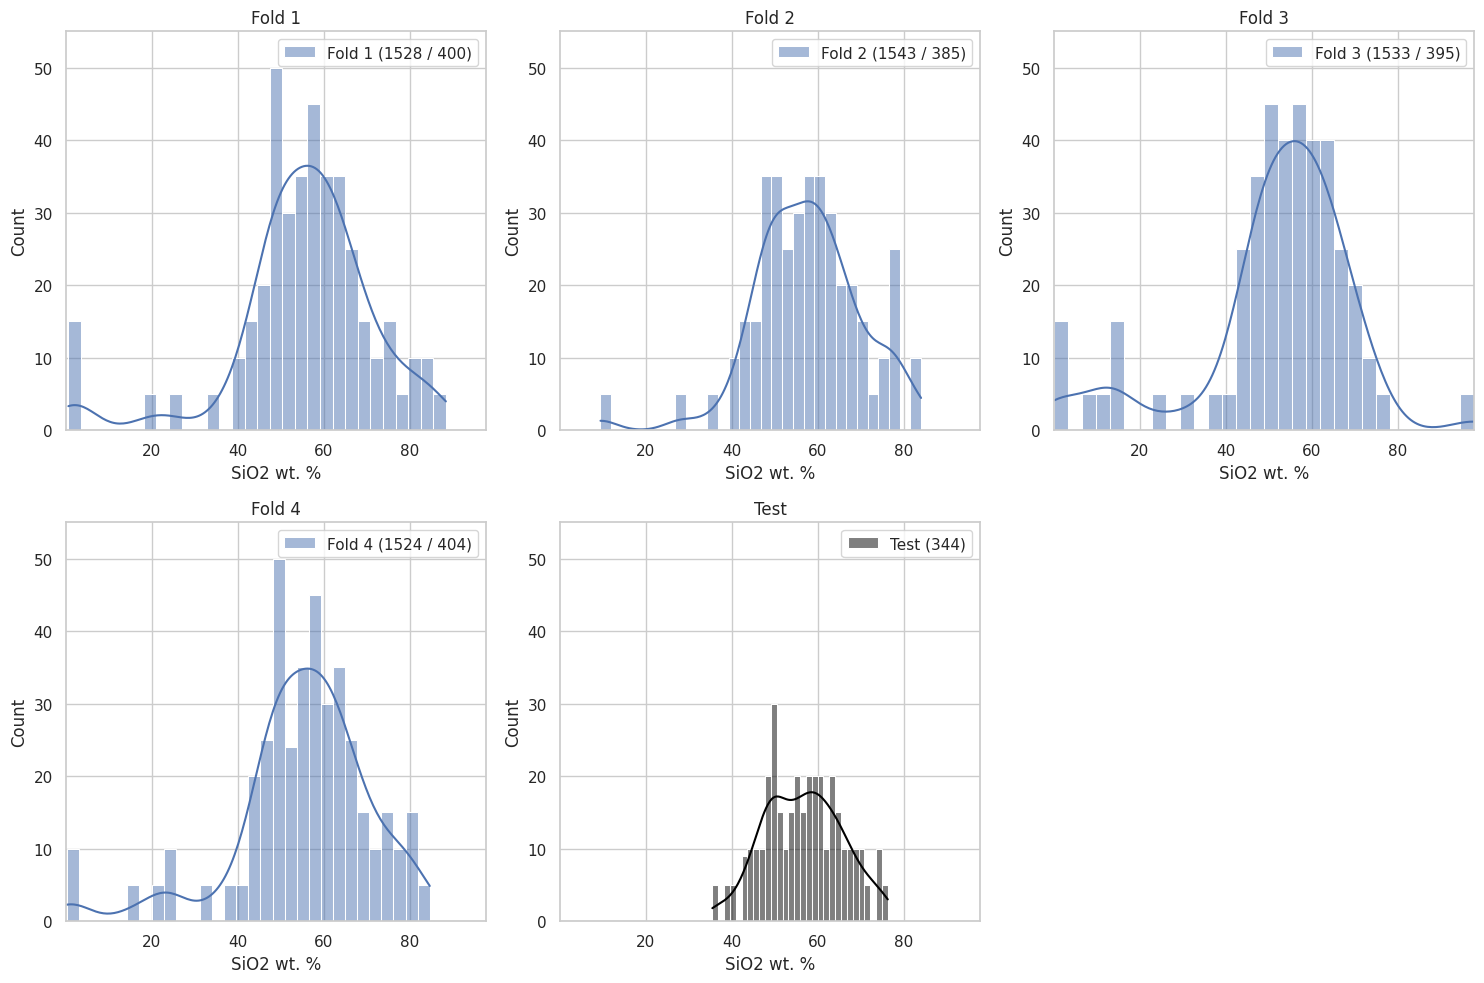
\includegraphics[width=\textwidth]{images/histogram_grid_plot.png}
    \caption{Histogram and \gls{kde} of \ce{SiO_2} Distribution in Each Fold.}
    \label{fig:histogram_grid_plot}
\end{figure*}

Figure \ref{fig:histogram_grid_plot} presents individual histograms and \gls{kde} curves for \ce{SiO_2} concentrations in each of the four cross-validation folds' validation sets and the full test set.
Each subplot shows the \ce{SiO_2} concentration (x-axis) against the count of samples per bin (y-axis).
The overlaid \gls{kde} curves provide a smoothed estimate of the probability density function for \ce{SiO_2} concentrations.

The histograms and \gls{kde} curves for each fold are remarkably similar, indicating that the data distribution within each fold closely matches the overall data distribution.
This similarity ensures that each fold is representative of the entire dataset, which is crucial for developing models that can generalize well.
The central tendency (mean) and spread (standard deviation) of \ce{SiO_2} concentrations appear consistent across all folds.
The \gls{kde} curves highlight that the density peaks and the tails of the distributions align well, suggesting that no fold is disproportionately skewed or biased.

These consistent distributions across folds validate our k-fold cross-validation method, confirming that each fold can provide a reliable estimate of model performance.
This balance helps in preventing overfitting, as the model is trained and validated on similarly distributed data in each fold.

\begin{figure*}[h!]
    \centering
    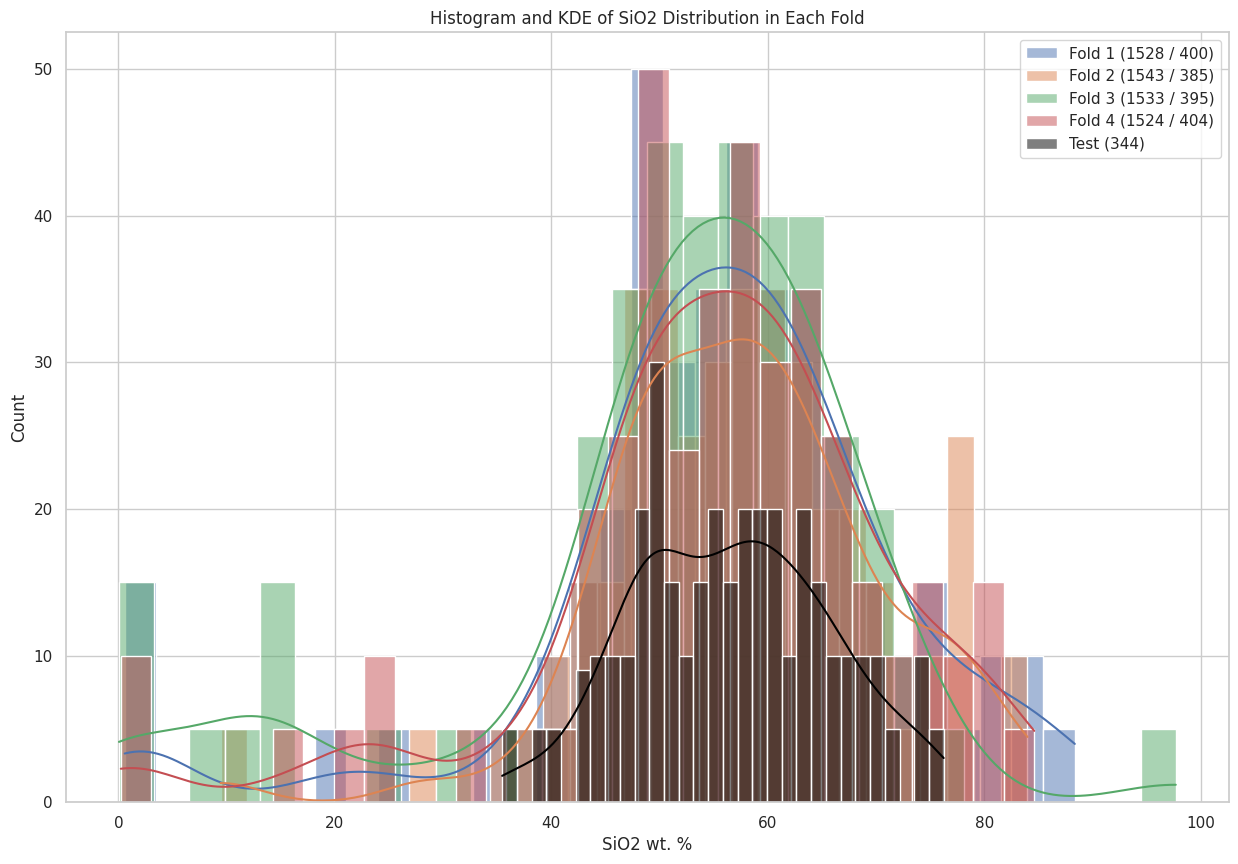
\includegraphics[width=\textwidth]{images/histogram_kde_plot.png}
    \caption{Combined Histogram and \gls{kde} of \ce{SiO_2} Distribution in Each Fold.}
    \label{fig:histogram_kde_plot}
\end{figure*}

Figure \ref{fig:histogram_kde_plot} combines the histograms and \gls{kde} curves of \ce{SiO_2} values from each fold and the full test set into a single plot, using different colors to represent each fold and the test set.
This visualization enables direct comparison of the distributions across the folds and the test set.

The combined histograms and \gls{kde} curves show a high degree of overlap, reinforcing the observation that the distributions are consistent across different folds and the test set.
The test set distribution closely follows the overall pattern observed in the folds, indicating that the test set is also representative of the overall dataset.
The presence of extreme values is evident in the tails of the distributions, particularly in the training folds.

\begin{figure*}[h!]
    \centering
    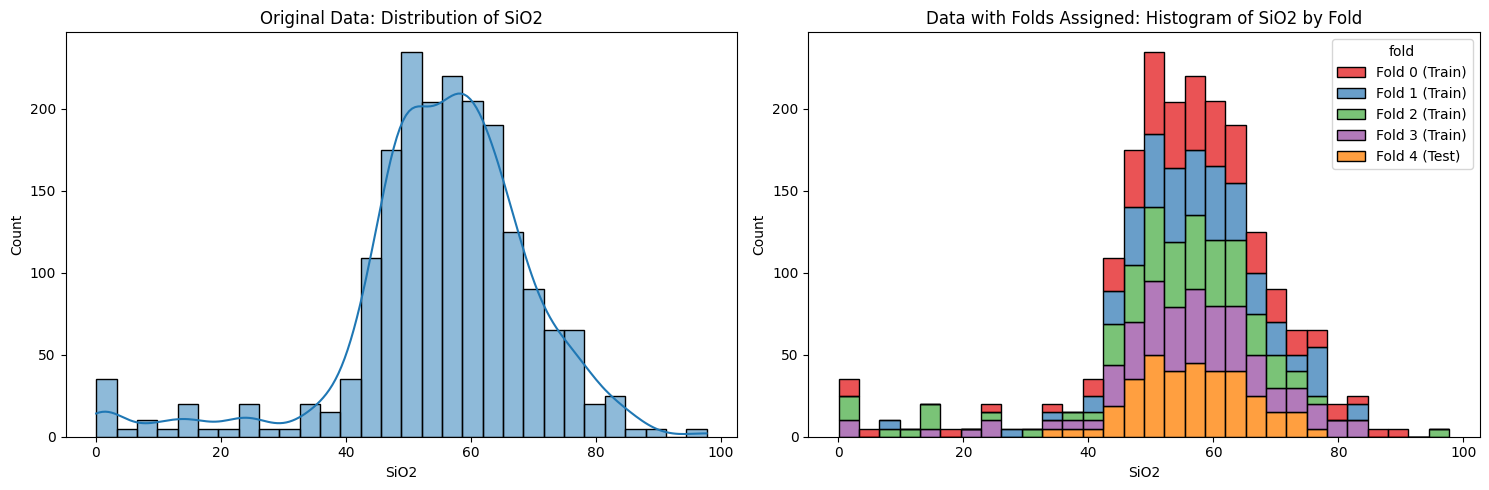
\includegraphics[width=\textwidth]{images/original_and_post_fold.png}
    \caption{Distribution of \ce{SiO_2} concentrations before and after fold assignment. The left plot shows the original distribution of \ce{SiO_2}, while the right plot shows the distribution with folds assigned, color-coded to indicate the different folds.}
    \label{fig:original_and_post_fold_plot}
\end{figure*}

Figure \ref{fig:original_and_post_fold_plot} contrasts the distribution of \ce{SiO_2} concentrations before and after the data partitioning process.
The left plot displays the original distribution of \ce{SiO_2} concentrations in the full dataset.
The right plot presents the distribution with assigned folds, using different colors to denote each fold.
This visualization highlights how the partitioning strategy maintains the overall data distribution while ensuring balanced representation across folds.

\subsubsection{Statistical Consistency}
To further validate our visual analysis, we can look at quantitative measures such as the means and standard deviations of \ce{SiO_2} concentrations across the folds and the overall dataset.
As shown in Table~\ref{tab:siO2_std_means}, the standard deviations and means for \ce{SiO_2} concentrations in each fold are as follows:

\begin{table}[h!]
    \centering
    \begin{tabular}{|c|c|c|}
        \hline
        \textbf{Fold} & \textbf{Standard Deviation} & \textbf{Mean} \\
        \hline
        Fold 1 & 16.28 & 55.70 \\
        \hline
        Fold 2 & 12.46 & 57.59 \\
        \hline
        Fold 3 & 18.01 & 51.51 \\
        \hline
        Fold 4 & 15.77 & 55.10 \\
        \hline
        Train Full & 15.91 & 54.96 \\
        \hline
        Test Full & 9.06 & 56.57 \\
        \hline
        Full & 14.94 & 55.25 \\
        \hline
    \end{tabular}
    \caption{Standard deviations and means of \ce{SiO_2} concentrations across different folds' validation sets, the full training set, the full test set, and the entire dataset.}
    \label{tab:siO2_std_means}
\end{table}

The means and standard deviations of \ce{SiO_2} concentrations for each fold are consistent with those of the overall dataset.
These metrics are even more similar across folds for the training sets, indicating that the training sets are also representative of the entire dataset.
This quantitative consistency supports the visual evidence that each fold is a reliable representative of the entire dataset.

\subsubsection{Importance of Distribution Balance}
Maintaining balanced and representative distributions in each fold is essential for training robust models.
It ensures that the models are not biased towards any specific subset of the data, which is crucial for their generalization to unseen data.
The balanced distributions across folds enable the model to be trained on diverse subsets of data, leading to better generalization.
This approach reduces the risk of overfitting and ensures that the model performs well on new, unseen data.

By ensuring that each fold is representative of the overall dataset, these visualizations validate our dataset partitioning strategy.
The consistency observed across folds supports the claim that the data distribution method works as intended, providing confidence in the generalizability and reliability of our models.

\subsubsection{Evaluation Metrics}\label{subsubsec:evaluation_metrics}
As mentioned in Section~\ref{sec:problem_definition}, the performance of the models was quantitatively assessed using the \gls{rmse} and the standard deviation of the residuals.
These metrics are calculated for each fold and averaged across all folds to provide comprehensive indicators of model accuracy and variability.
In addition, we also compute the metrics for the test set to provide a measure of the model's performance on unseen data.
Therefore, we have the following metrics for each experiment:
\begin{enumerate}
    \item \textbf{Fold-specific \gls{rmse} and Standard Deviation:} For each of the $k$ folds, we calculate both the \gls{rmse} and standard deviation, denoted as \texttt{rmse\_cv\_n} and \texttt{std\_dev\_cv\_n}, where \texttt{n} ranges from 1 to $k$.
    \item \textbf{Average \gls{rmse} and Standard Deviation:} The overall cross-validation \gls{rmse} (\texttt{rmse\_cv}) and standard deviation (\texttt{std\_dev\_cv}) are computed as the mean of the fold-specific values.
    \item \textbf{Test Set \gls{rmse} and Standard Deviation:} The \gls{rmse} and standard deviation are also computed for the test set, denoted as \texttt{rmsep} and \texttt{std\_dev}, to provide a measure of the model's performance on unseen data.
\end{enumerate}

K-fold cross-validation provides a robust estimate of model performance by averaging metrics over multiple folds, reducing variance and offering a clearer picture of the model's generalizability.
Evaluating the model on a separate test set representative of unseen data ensures that performance metrics accurately reflect the model's generalization capability.
However, our data partitioning method, which moves the most extreme values into the training data, naturally results in the testing data being closer to the mean of the data distribution, making it easier to predict.
In practice, this would result in lower \texttt{rmsep} and \texttt{std\_dev} values compared to the cross validation metrics.
Therefore, evaluating the model's performance using both the cross-validation metrics (\texttt{rmse\_cv} and \texttt{std\_dev\_cv}) and the test set metrics (\texttt{rmsep} and \texttt{std\_dev}) is crucial.
The cross-validation metrics provide insights into the model's stability across different subsets, while the test set metrics offer a final measure of performance on truly unseen data, giving a comprehensive assessment of the model's generalizability.


\subsubsection{Conclusion}
In summary, our validation and testing procedures are designed to ensure the robustness and generalizability of our models by employing a combination of k-fold cross-validation and a separate test set.
The customized k-fold cross-validation algorithm mitigates data leakage by ensuring that data points from the same target are not split across training and testing sets.
This method, which includes handling extreme values, aligns with established practices and optimally partitions the dataset to maintain a balance between representativeness and model training efficacy.
By assessing model performance through metrics such as \gls{rmse} and standard deviation across both cross-validation folds and a separate test set, we provide an evaluation framework that underscores the reliability and accuracy of our predictive models.

